\section{Experimentales Setup}


\subsection{Hardware}
Server mit 4 Graka:

2 mal Geforce GTX 1080 Ti mit CUDA Version 10.1 

2 mal Geforce RTX 2080 Ti mit CUDA Version 10.1

\subsection{Wahl des Frameworks}

Es wird mit pytorch gearbeitet, da pytorch gegenüber anderen Frameworks eine grössere Flexibiltät erlaubt. Ausserdem ist eine fast vollständige Implementierung von PruneTrain in Pytorch geschrieben. Diese wird im nächsten Kapitel untersucht und soweit erweitert, dass es dem Stand im PruneTrain Paper entspricht.

Pytorch bietet mit cudnn und cuda im Hintergrund gute Möglichkeiten die Trainingszeiten einzelner Epochen zu messen und sie so mit einander zu vergleichen.


\subsection{verwendete Netzarchitektur}\label{sec:archi}
Die PruneTrain Implementierung hat initial mehrere verschiedene Netzarchitekturen zur Auswahl:
\begin{itemize}
 \item AlexNet
 \item ResNet 32/50
 \item vgg 8/11/13/16
 \item mobilenet
\end{itemize}

Schränke diese Auswahl auf ResNet ein.
Gründe hierfür:
\begin{itemize}
 \item Da die Überlegung besteht diese Netze tiefer zu machen wähle ResNet, da die Identity-Übergänge dem Netz erlauben das degradation Problem zu umgehen während das Netz noch tiefer/ breiter wird.
 \item Festlegung auf eine Architektur um Umfang der Arbeit zu begrenzen
\end{itemize}

Erweitere dies jedoch durch beliebige grosse ResNets. Ein ResNet ist hier durch 4 Parameter charaterisiert:

\begin{itemize}
 \item $s$: Anzahl an Stages, die das ResNet hat
 \item $[n]:$ Anzahl von Blöcken pro Stage 
 \item $l$: Anzahl von (Conv+Batch)-Layer pro Block
 \item $b$: Boolean Parameter, der angibt ob die Blöcke im Netz die Bootleneck-Eigenschaft haben
\end{itemize}
\todo[inline]{Bottleneck -Eigenschaft}
\subsection{Überblick über das experimentelle Vorgehen}


\section{Untersuchung von PruneTrain}

Die Untersuchung von PruneTrain basiert auf einer bereits vorgefertigten Implementierung \cite{ptImpl}. 

\subsection{Evaluation von PruneTrain}

Hier wird das Ergebnis der Ausführung von PruneTrain auf der Hardware mit den Ergebnissen aus dem Prune Train Paper verglichen. Im ersten Abschnitt wird zunächst betrachtet, wie sich die Trainingszeiten bei den veränderbaren Hyperparametern von PruneTrain verändern. Im zweiten Abschnitt wird betrachtet, wie sich die Accuracy im Verlauf der Epochen verhält.

Als Netzwerk wird ein Res-Net 32 verwendet. In Tabelle \todo{ref} ist die Netzstruktur aufgeführt.



verwendete Kenngrößen:

\begin{itemize}
 \item 1 GPU
 \item Cifar10
 \item 180 Epochen
\end{itemize}

Zunächst wird hierfür nur das Prune Train ohne Anpassung der Batchgrösse betrachtet. 

Variable Größen, die in verschiedenen Experimenten geändert werden:

\begin{itemize}
 \item Lernrate
 \begin{itemize}
  \item unterschiedlich große Lernraten
  \item Anpassung der Lernrate währenddem Training
 \end{itemize}

 \item Rekonfigurationsinterval
 \item Threshold
 \item Lasso-Ratio
 \item Batchgröße:
 \begin{itemize}
  \item unterschiedliche Batchgrößen verschiedener Durchläufen
  \item Anpassung der Batchgröße währenddem Training
 \end{itemize}
\end{itemize}

Um die Experimente mit den unterschiedlich großen Kenngrößen vergleichen zu können wird jeweils eine Größe geändert und der Einfluss dieser Größe auf die Trainingszeit betrachtet. Betrachte zunächst eine feste Batchgröße von 256 über alle 180 Epochen und vergleiche diese mit mehreren Durchläufen des Baseline-Netzes. 
\subsubsection{Experimente zur Lernrate}

Die Trainingszeiten in Sekunden pro Epoche für verschiedene Lernrate ist in Abbildung \ref{abb:lr} zu sehen. Unterschiede zwischen den Experimente sind in Abbildung \ref{abb:lr1} zunächst nicht direkt sichtbar. Um diese besser sichtbar zu machen wird für jedes Experimente die Summeder Trainingszeiten über die Epochen gebildet. In Abbildung \ref{abb:lr2} ist zu beobachten, dass beim größten Threshold die geringste summierte Trainingszeit zusammenkommt. Da bei einem höheren Threshold im Laufe des Trainings mehr Gewichte unter den Grenzwert fallen und somit entfernt werden. Liegen diese Gewichte sinnvoll, so können ganze Kanäle entfernt werden.
 \begin{figure}[h]
 \centering
 \subfloat[][verschiedene Experimente]{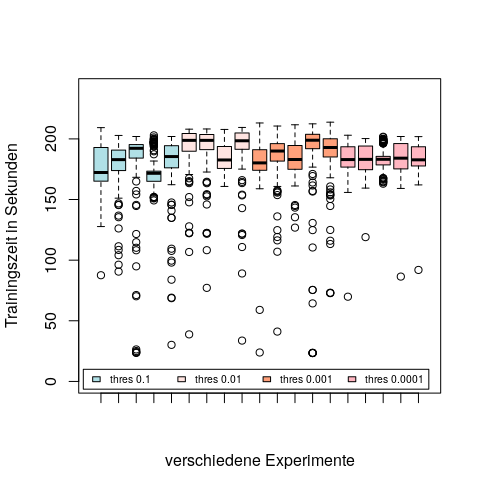
\includegraphics[width=0.37\textwidth]{KapitelPartB/Images/thres1.png}\label{abb:lr1}}
 \qquad
 \subfloat[][Summe verschiedener Experimentengruppen]{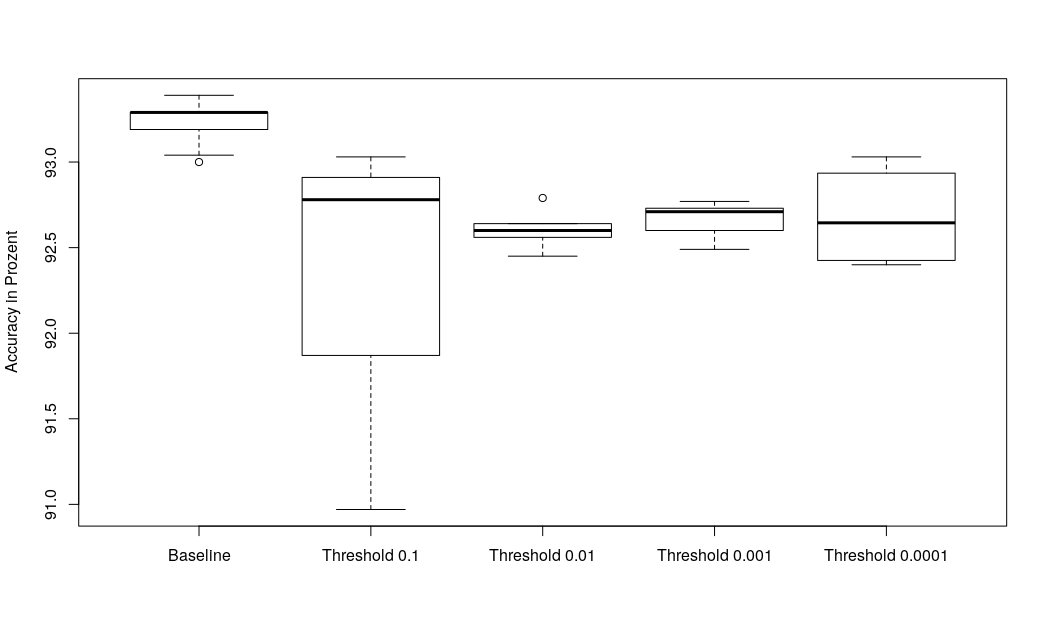
\includegraphics[width=0.55\textwidth]{KapitelPartB/Images/thres2.png}\label{abb:lr2}}
 \caption{Boxplot der verschiedenen Grenzwerte}
 \label{abb:lr}
\end{figure}
 
 In Abbildung \ref{abb:lr3} ist zu sehen, dass der gleiche Effekt sich auch bei Accuracy zeigt. Die Accuracy für den größten Grenzwert ist am niedrigsten.
 
 \begin{figure}[h]
 \centering
 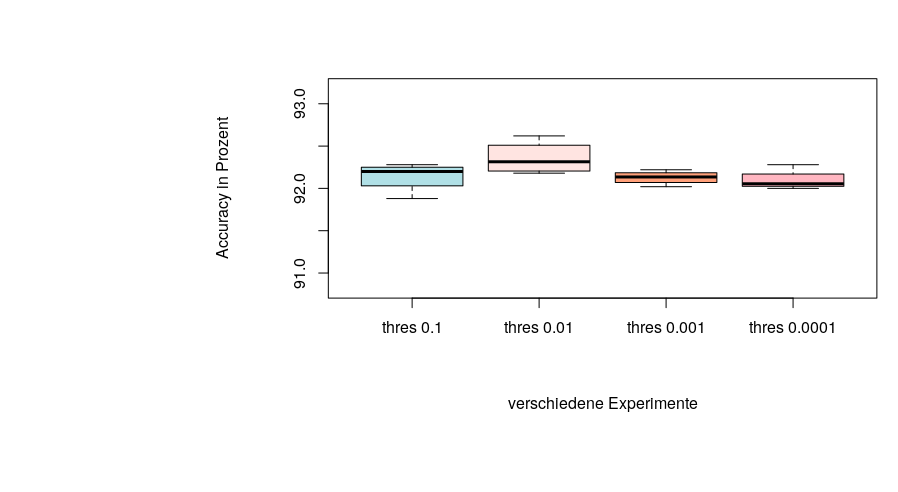
\includegraphics[width=0.8\textwidth]{KapitelPartB/Images/thres3.png}
 % reconf3.png: 454x491 px, 96dpi, 12.01x12.99 cm, bb=0 0 341 368
 \caption{Accuracy von verschiedenen Experimentengruppen des Grenzwerts}
 \label{abb:lr3}
 \end{figure}


\subsubsection{Experimente zum Rekonfigurationsintervall}

 Als nächste Größe wird der Einfluss des Rekonfigurationsintervalls überprüft. Die entsprechenden Grafiken sind in Abbildung \ref{abb:reconf} abgebildet. In Abbildung \ref{abb:reconf1} sind für die verschiedenen Experimente die Trainingszeiten pro Epoche zu sehen. Dabei werden drei verschiedene Rekonfigurationsintervalle (2,5 und 10) verglichen. In Abbildung \ref{abb:reconf1} lässt sich für die verschiedenen Experimente keine großen Unterschiede sehen. Werden die Zeiten der jeweiligen Experimente addiert und in einem Boxplot dargestellt entsteht Abbildung \ref{abb:reconf2}. In dieser Abbildung ist deutlich zu sehen, dass mit steigendem Rekonfigurationsintervall auch die Summe der Trainingszeiten pro Epoche steigt.
 
 \begin{figure}[h]
 \centering
 \subfloat[][verschiedene Experimente]{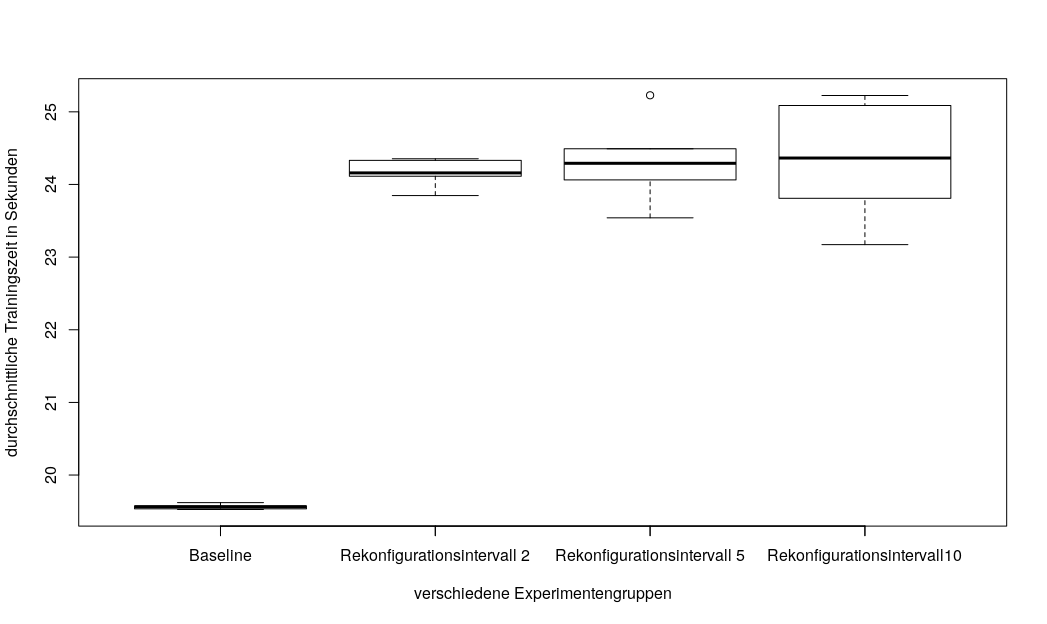
\includegraphics[width=0.47\textwidth]{KapitelPartB/Images/reconf1.png}\label{abb:reconf1}}
 \qquad
 \subfloat[][Summe verschiedener Experimentengruppen]{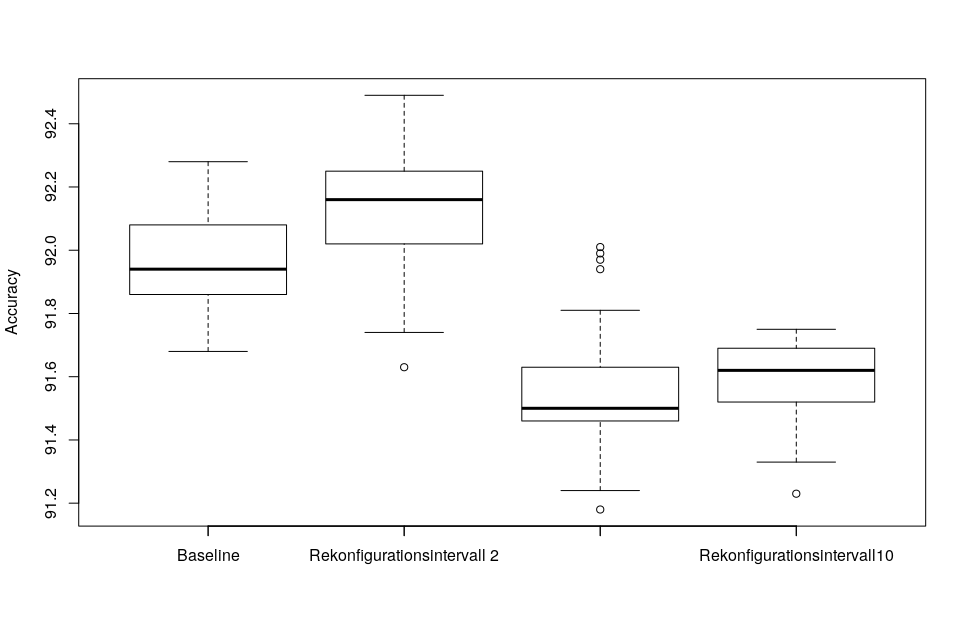
\includegraphics[width=0.47\textwidth]{KapitelPartB/Images/reconf2.png}\label{abb:reconf2}}
 \caption{Boxplot der Rekonfigurationsintervalle}
 \label{abb:reconf}
\end{figure}

 Dies bedeutet, dass der Overhead des Beschneidungsverfahrens geringer ist als der Gewinn durch das Verkleinern des Netzes. In Abbildung \ref{abb:reconf3} ist zu sehen, dass dieser Gewinn an Trainingszeit in Abbildung \ref{abb:reconf2} mit einem Verlust an geringem Verlust an Accuracy einhergeht.  

 
 \begin{figure}[h]
 \centering
 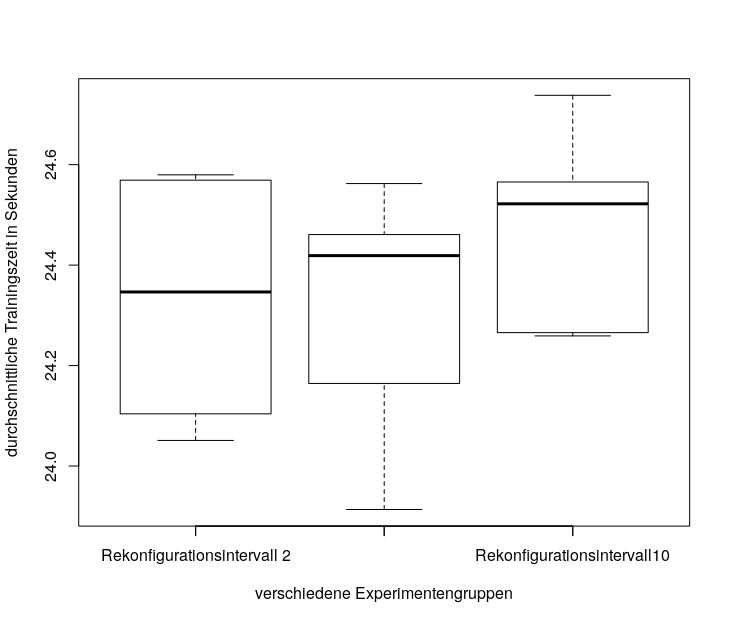
\includegraphics[width=0.5\textwidth]{KapitelPartB/Images/reconf3.png}
 % reconf3.png: 454x491 px, 96dpi, 12.01x12.99 cm, bb=0 0 341 368
 \label{abb:reconf3}
 \caption{Accuracy von verschiedenen Experimentengruppen des Rekonfigurationsintervall}
\end{figure}

 \subsubsection{Experimente zum Grenzwert}


\begin{figure}[h]
 \centering
 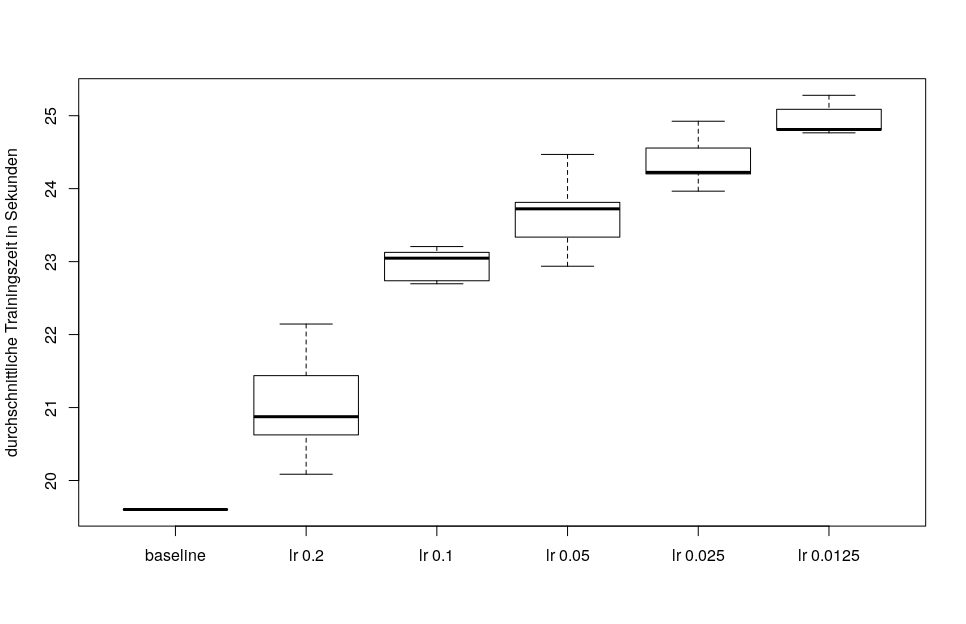
\includegraphics[width=0.8\textwidth]{KapitelPartB/Images/lr1.png}
 % lr1.png: 431x491 px, 96dpi, 11.41x12.99 cm, bb=0 0 323 368
 \label{ref:lra}
\end{figure}

 In Abbildung \ref{abb:lra} ist nicht wirklich was zu sehen, 
 
 
 
Es ergibt sich, dass sich mit diesen bisherigen Experimenten keine Zeit sparen lässt. Im Gegenteil, der PruneTrain Ansatz braucht mehr Zeit. Dies steht im Widerspruch zum PruneTrain Paper. Dieser Widerspruch lässt sich durch die Verwendung von mehreren GPUs zur Evaluation im PruneTrain Paper erklären. Mit einem schmalleren Netz müssen weniger Daten zwischen den GPUs ausgetauscht werden. Es wird Kommunikationszeit gespart.




\todo[inline]{Bis hier muss noch mit mehr Experimenten sichergestellt werden, dass die Effekte nicht an der kleinen Zahl an Experimenten liegt.}
\color{blue1}

\subsubsection{Experimente zur Batchgröße}



Gleichzeitig wird für die jeweilige Modellgrösse die Anzahl an Parametern, die das Modell hat gezählt. Diese Größen sind in Tabelle \ref{tab:batchSize} eingetragen. 


Mit Hilfe dieser Grössen wird für jede einzelne Stagegröße eine Gerade gefittet.

Diese gefittete Gerade wird mittels t-Test darauf überprüft wie wahrscheinlich beim Fitten der Gerade ein Fehler 1. Art auftritt.

Hierfür werden folgende Hypothesen aufgestellt:


Da der p-Wert für diese Gerade bei $p=2,911e^{-16}$ und damit weit unter de Signifikanzniveau von $\alpha=0,05$ kann die $H_0$ Hypothese abgelehnt werden und die Alternativhypothese angenommen werden.

Dies bestätigt statistisch eine hohe Wahrscheinlichkeit, dass die gefittete Gerade richtig ist.



In Abbildung \ref{fig:linearBlocks} ist zu sehen, dass die Parameteranzahl in Zusammenhang mit der Anzahl an Blöcken linear steigt.
Wird das Netz kleiner, so kann anhand der Gerade abhängig von der Parameteranzahl die neue Batchgröße errechnet werden.






\todo{beispielrechnung}

In Abbildung \todo{ref} ist abgebildet. wie sich die Trainingszeiten verändern, wenn die Batchgrösse angepasst wird.



\subsubsection{Veränderung der Accuracy durch PruneTrain}

Durch das Pruning währenddem Training wird die Accuracy kleiner. In Abbildung \ref{abb:PTaccuracy} ist zu sehen wie sich im Accuracy im Verlauf der Epochen verändert.  

\begin{figure}[h]
 \centering
 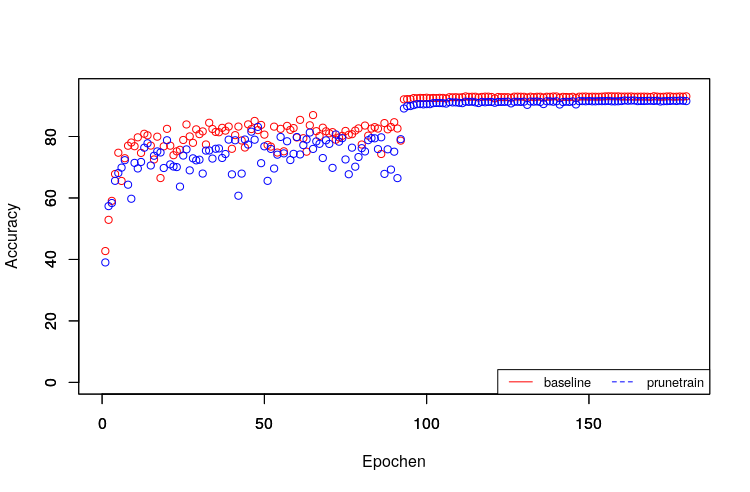
\includegraphics[width=0.8\textwidth]{KapitelPartB/Images/PTaccuracy.png}
 % PTaccuracy.png: 750x492 px, 96dpi, 19.85x13.02 cm, bb=0 0 563 369
 \caption{Veränderung der Accuracy während der Epochen}
 \label{abb:PTaccuracy}
\end{figure}

In Abbildung \ref{abb:PTaccuracyzoom} sind die Epochen 90 bis 180 näher herangezoomt.

\begin{figure}[h]
 \centering
 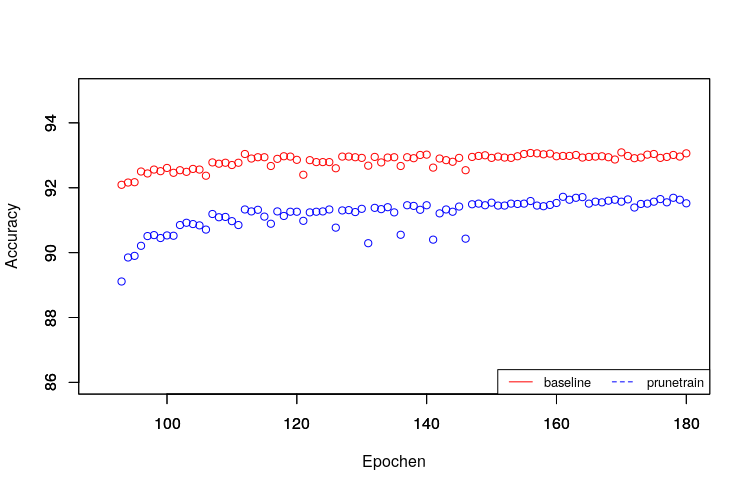
\includegraphics[width=0.8\textwidth]{KapitelPartB/Images/PTaccuracyzoom.png}
 % PTaccuracyzoom.png: 750x492 px, 96dpi, 19.85x13.02 cm, bb=0 0 563 369
 \caption{Zoom der Veränderung}
 \label{abb:PTaccuracyzoom}
\end{figure}

Man sieht eine geringere Accuracy von PruneTrain im Vergleich zum Baseline. Diese Verringerung der Accuracy lässt sich durch ein Aussetzen des Verkleinern des Netzes in den letzten Epochen  
vermindern.

Die Frage die sich hier stellt ist, ob diese Verminderung der Accuracy am Ende der dieser Arbeit noch ins Gewicht fällt. Wenn mit Hilfe einer Kombination von MorphNet und PruneTrain ein bessere Architektur gefunden wird kann diese Architektur auch direkt mit Hilfe des äquivalenten Baseline Netzes berechnet werden.

\subsection{Einfluss der Batchgröße auf PruneTrain}\label{sec:batch}

Das heisst es ist nötig, zu wissen wie gross die Batches maximal sein dürfen um keinen Out of Memory Error zu provozieren. Zusätzlich kann dann berechnet werden, inwieweit die Batchgrösse weiter angehoben werden kann bei kleiner werdendem Netz

Um die Anpassung der Batchgröße an die Verkleinerung des Netzwerkes durch das Prunen zu implmentieren muss zunächst die Batchgröße des Ausgangsnetzes so gewählt werden, dass der GPU-Speicher maximal ausgelastet ist.



Theoretisch sollte hierfür nachdem Übertragen des Modells der freie Speicher ausglesen werden und anhand des Speicherverbrauchs eines Elements des Datensatzes berechnet werden, wie gross die Batchgröße maximal sein darf. Leider führt diese Methode nicht zum gewünschten Ergebnis, da der ausgelesene freie Speicher nicht dem tratsächlich allokierbaren Speicher entspricht.
Der Grund hierfür ist ein Fragmentierungsproblem. Verschiedene freie Blöcke können nicht zu einem grossen allokierbaren Block zusammengefügt werden.\todo[inline]{Quelle}. 

Diese Problem wird mit einer Methode, die für einen beliebigen Datensatz und für eine beliebige Modellgrösse die maximale Batchgröße berechnet, gelöst. 


\todo[inline]{Tabelle mit neuen Zahlen updaten, da mit kaputter Grafikkarte berechnet}
\begin{table}[]
\begin{tabular}{c|c|c|c|c|c|c|c|c|}
\cline{2-9}
                         & \multicolumn{2}{c|}{s=1}  & \multicolumn{2}{c|}{s=2}  & \multicolumn{2}{c|}{s=3}  & \multicolumn{2}{c|}{s=4}  \\ \cline{1-1}
\multicolumn{1}{|l|}{}   & \#Para & Batch & \#Para & Batch & \#Para & Batch & \#Para & Batch \\ \hline
\multicolumn{1}{|l|}{1}  & 7642         & 14272      & 31034        & 5856       & 123898       & 2704       & 493946       & 1344       \\ \hline
\multicolumn{1}{|l|}{2}  & 14650        & 8816       & 65882        & 3328       & 269722       & 1472       & 1082906      & 688        \\ \hline
\multicolumn{1}{|l|}{3}  & 21658        & 6512       & 100730       & 2368       & 415546       & 1024       & 1671866      & 480        \\ \hline
\multicolumn{1}{|l|}{4}  & 28666        & 5072       & 135578       & 1808       & 561370       & 784        & 2260826      & 368        \\ \hline
\multicolumn{1}{|l|}{5}  & 35674        & 4208       & 170426       & 1488       & 707194       & 624        & 2840786      & 288        \\ \hline
\multicolumn{1}{|l|}{6}  & 42682        & 3568       & 205274       & 1232       & 853018       & 528        & 3438746      & 240        \\ \hline
\multicolumn{1}{|l|}{7}  & 49690        & 3120       & 240122       & 1072       & 998842       & 464        & 4027706      & 208        \\ \hline
\multicolumn{1}{|l|}{8}  & 56698        & 2736       & 274970       & 944        & 1144666      & 400        & 4616666      & 176        \\ \hline
\multicolumn{1}{|l|}{9}  & 63706        & 2464       & 309818       & 848        & 1290490      & 352        & 5205626      & 160        \\ \hline
\multicolumn{1}{|l|}{10} & 70714        & 2224       & 344666       & 752        & 1436314      & 320        & 5794586      & 145        \\ \hline
\multicolumn{1}{|l|}{11} & 77722        & 2049       & 379514       & 688        & 1582138      & 288        &              &            \\ \hline
\end{tabular}
\end{table}




\begin{figure}[h]
 \centering
 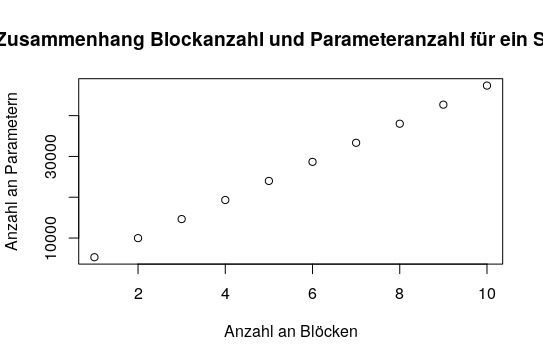
\includegraphics[width=0.8\textwidth]{KapitelPartB/Images/linearBlocks.png}
 % batchSizevsTime.png: 387x367 px, 96dpi, 10.24x9.71 cm, bb=0 0 290 275
 \caption{Batch Size vs Trainings Time über eine Epoche}
 \label{fig:linearBlocks}
\end{figure}




Die maximal mögliche Batchgrösse in Abbildung \ref{fig:maxBatchSize} sinkt im Gegensatz dazu stärker als linear bei mehr Blöcken im Netz. Dies liegt darin begründet, dass für ein grösseres Netz mehr Werte zwischengespeichert werden müssen, was den Speicherbedarf erhöht.

\begin{figure}[h]
 \centering
 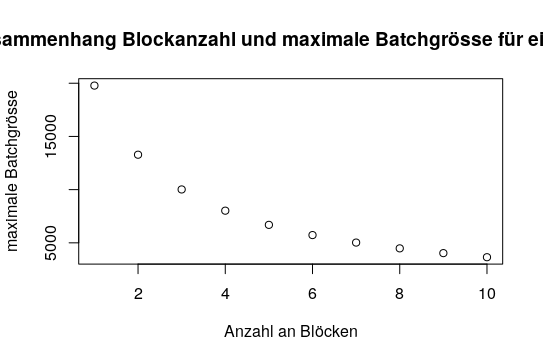
\includegraphics[width=0.8\textwidth]{KapitelPartB/Images/maxBatchSize.png}
 % batchSizevsTime.png: 387x367 px, 96dpi, 10.24x9.71 cm, bb=0 0 290 275
 \caption{Batch Size vs Trainings Time über eine Epoche}
 \label{fig:maxBatchSize}
\end{figure}




Gesucht ist ein idealerweise linearer Zusammenhang zwischen der Parameteranzahl und der Batchgrösse. Um diesen herzustellen wird die Parameteranzahl durch die Batchanzahl geteilt. Das Ergebnis hiervon ist in Abbildung \ref{fig:quotient} zu sehen.

\begin{figure}[h]
 \centering
 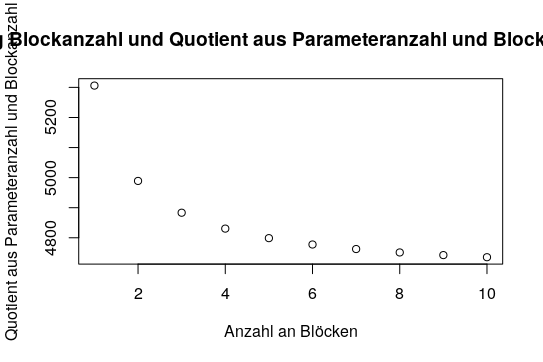
\includegraphics[width=0.8\textwidth]{KapitelPartB/Images/quotient.png}
 % batchSizevsTime.png: 387x367 px, 96dpi, 10.24x9.71 cm, bb=0 0 290 275
 \caption{Batch Size vs Trainings Time über eine Epoche}
 \label{fig:quotient}
\end{figure}


Da diese Kurve ähnlich der Batchsize-Kurve aussieht wird die Hypothese untersucht, ob hier ein linearer Zusammenhang besteht. Zu diesem Zweck wird die Batchgrösse durch das Ergebnis geteilt.

Augenscheinlich liegt hier ein linearer Zusammenhang vor. Daher wird hier eine Gerade gefittet.
Es entsteht die Abbildung \ref{fig:gerade}.

\begin{figure}[h]
 \centering
 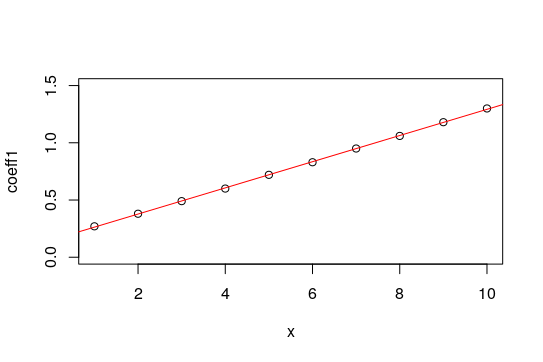
\includegraphics[width=0.8\textwidth]{KapitelPartB/Images/gerade.png}
 % batchSizevsTime.png: 387x367 px, 96dpi, 10.24x9.71 cm, bb=0 0 290 275
 \caption{Batch Size vs Trainings Time über eine Epoche}
 \label{fig:gerade}
\end{figure}




Die gefittete Gerade hat die Gleichung: $$ f(x)=0.11 \cdot x +  0.15 $$

\todo{Hier muss noch das Fitten des Modells und der t-Test erklärt werden}

In Tabelle \todo{Tabelle} werden die Werte für die anderen Stages zusammengefasst. Zu sehen ist, dass für jeden Stage die gefittete Gerade ähnlich im t-Test abschneidet.







Als nächsten Schritt wird untersucht wie das Intervall wie häufig rekonfiguriert wird den Zusammenhang zwischen Inferenz Flop und der Validation Accuracy verändert.


Die nächste Untersuchung über das Sparen von Kommunikationskosten beim Verteilten Training macht hier keinen Sinn da nur eine einzelne Graka genutzt wird.


Abschliessend wird noch evaluiert, wie die Dichte der Gewichte mit der Dichte der Kanäle nachdem Training zusammenhängen um eventuell durch spezifische Inferenzhardware weiter zusparen.





Bei grösserer Batchgrösse wird auch das Netz schneller. Dies ist in Abildung \ref{fig:batchVsTime} für das ResNet und die verwendete Hardware abgebildet.

\begin{figure}[h]
 \centering
 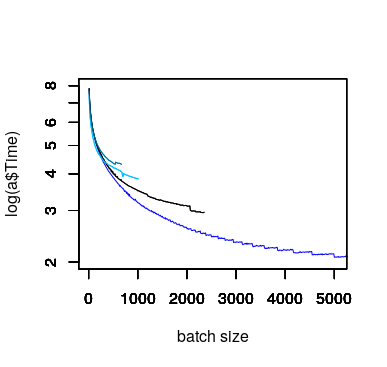
\includegraphics[width=0.8\textwidth]{KapitelPartB/Images/batchSizevsTime.png}
 % batchSizevsTime.png: 387x367 px, 96dpi, 10.24x9.71 cm, bb=0 0 290 275
 \caption{Batch Size vs Trainings Time über eine Epoche}
 \label{fig:batchVsTime}
\end{figure}


Wie zu sehen ist, wird die Trainingszeit pro Epoche mit grösserer Batchgrösse kleiner. Die höhere Batchgrösse sorgt neben der geringeren Trainingszeit auch für weniger Gewichtsupdates. Dies führt zu einer geringeren Generalisationsfähigkeit und damit zu einer geringeren Klassifikationsleistung \cite{largeBatch}. Um diesen Verlust an Klassifikationsleistung auszugleichen gibt es die Möglichkeit die Lernrate anzupassen und eine andere Batch Normalisation zu verwenden \cite{largeBatch}. Diese Technik funktioniert laut dem Paper "`Train longer, generalize better: closing the generalization gap in large batch training of neural networks"' bereits auf residualen Netzen wie sie in dieser Arbeit verwendet werden \cite{largeBatch}. Vorallem bleibt die Einsparung bei der Trainingszeit durch diese Technik intakt \cite{largeBatch}.

Ist dieser Effekt auf PruneTrain übertragbar?


Eine grössere Batchsize sorgt auf jeden Fall für signifikant weniger Verkleinerung des Netzes.
\todo{t-Test um statistisch zu zeigen, dass das signifikant ist}

Die Frage die sich hier stellt ist, ob mit Hilfe von largeBatch bei maximaler Batchsize die Verkleinerungsrate steigt  


\subsubsection{Ghost Batch Norm und LR Anpassung}

\subsubsection{Untersuchung}
Im nächsten Schritt wird untersucht, ob diese Vorteile auch für den PruneTrain Vorgang genutzt werden kann. Dafür wird zunächst untersucht, welchen Effekt eine grössere Batchgrösse auf PruneTrain hat.




Es stellt sich die Frage, ob das einen so grossen Einfluss auf die Ausführungszeit hat.



Man sieht, dass mit steigender Batchgröße die Ausführungszeit sinkt. 

Errechne zusätzlich noch ein Modell, wo abhängig von der Modellgrösse währenddem Pruning die Batchgrösse angepasst wird.



\cite{largeBatch} gibt an, dass mit grösserer Batch size die Accuracy weniger wird. Aber dort wird ein Verfahren angegben, welches diesen Effekt entfernen kann.
Da dieser Effekt da sehr deutlich gezeigt wird hier im nächsten Unterkapitel nur die Überprüfung, ob dieser Effekt auf bei geprunten Netzwerken funktioniert.
\subsection{Einfluss der Batchgrösse und der Lernrate auf die Verkleinerung des Netzes}
\todo[inline,color=blue]{Untersuche, ob largeBatch auch auf ein PruneTrain Netzwerk anwendbar ist.}
\todo[inline,color=brown]{Untersuche, ob die Grösse des Batches beeinflusst, wie viel vom Netz geprunt wird}



\section{Untersuchung von Net2Net}


\section{Untersuchung von MorphNet}

MorphNet macht alle Layer breiter um sie dann mit einem speziellen Regularisierer breiter zu machen. Dieser Regularisierer hat verschiedene mögliche Zielgrössen (Modelgrösse, Flops oder Inferenz-Zeit).
Die Frage stellt sich hier, ob das Netz besser wird wenn alle Schichten breiter gemacht werden um später wieder geprunt zuwerden.

Weiterhin besteht die Möglichkeit das Netz nicht nur breiter zu machen sondern auch tiefer.


MorphNet erwähnt, dass es Sinn macht nicht im ganzen Netz denn Wider Operator anzuwenden sonder nur da wo der Regularisierer das Netz nicht schmaller macht.
\section{PruneTrain + Net2Net}

\section{Additive Verfahren}

\subsection{Zahlenformate}

\begin{itemize}
 \item FP16 bereits probiert
\end{itemize}


FP16 nur auf RTX 2080 sinnvoll
Bietet nach erster Messung etwa 28 \% Prozent Gewinn.

Code für dieses Verfahren liegt vor: Amp apex von Nvidia

AMP bietet 3 mögliche Optimierungsstufen:

O1
Patch all Torch functions and Tensor methods to cast their inputs according to a whitelist-blacklist model. Whitelist ops (for example, Tensor Core-friendly ops like GEMMs and convolutions) are performed in FP16. Blacklist ops that benefit from FP32 precision (for example, softmax) are performed in FP32. O1 also uses dynamic loss scaling, unless overridden.

02
casts the model weights to FP16, patches the models forward method to cast input data to FP16, keeps batchnorms in FP32, maintains FP32 master weights, updates the optimizer’s paramgroups so that the optimizer.step() acts directly on the FP32 weights (followed by FP32 master weight-FP16 model weight copies if necessary), and implements dynamic loss scaling (unless overridden). Unlike O1, O2 does not patch Torch functions or Tensor methods.


O3
may not achieve the stability of the true mixed precision options O1 and O2. However, it can be useful to establish a speed baseline for your model, against which the performance of O1 and O2 can be compared. If your model uses batch normalization, to establish speed of light you can try O3 with the additional property override keepBatchnormfp32=True (which enables cudnn batchnorm, as stated earlier).

Hier nur O0, O1 und O2 dargestellt, da O3 absolut nicht mithalten kann was Performance angeht.

\begin{figure}[h]
 \centering
 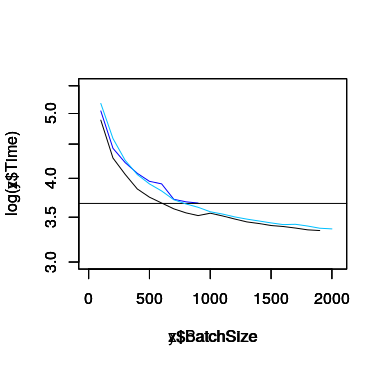
\includegraphics[width=0.8\textwidth]{KapitelPartB/Images/timeVsBatchSize_Amp.png}
 % timeVsBatchSize_Amp.png: 387x367 px, 96dpi, 10.24x9.71 cm, bb=0 0 290 275
 \caption{Vergleich Trainingszeit einer Epoche für verschiedene Optimierungsstufen von Amp Apex. DunkelBlau=O0; Schwarz = O1; Hellblau=O2}
 \label{fig:amp}
\end{figure}

\todo[inline,color=brown]{Weitere Versuche, die zeigen ob die Zeiten grossen statistischen Schwankungen unterliegen.}
\url{https://developer.download.nvidia.com/video/gputechconf/gtc/2019/presentation/s9998-automatic-mixed-precision-in-pytorch.pdf} zeigt, dass bezüglich der Accuracy kein Verlust zu erwarten ist.

Da O2 gegenüber O1 keinen signifikanten zusätzlichen Gewinn bringt nutze O1.
\subsection{Beschleunigung der Berechnung des Gradientenabstiegverfahren}


Accelerating CNN Training by Sparsifying Activation Gradients funktioniert nur auf Toy-Benchmarks 


\subsubsection{Weight Normalization: A Simple Reparameterization
to Accelerate Training of Deep Neural Networks}

\todo[inline,color=blue]{Testen ob es funktioniert}
Könnte funktionieren. Code für Lasagne: https://github.com/TimSalimans/weight\_norm


\subsubsection{Accelerating Deep Neural Network Training with Inconsistent Stochastic Gradient Descent}

Interessant bisher kein Code verfügbar
\todo[inline, color=blue]{Implementieren (ist einfach) und testen}

\subsubsection{Accelerated CNN Training Through Gradient Approximation }

Interessant bisher kein Code verfügbar


